\documentclass[a4paper]{article}
\usepackage{xeCJK}
\usepackage{geometry}
\geometry{left=2.5cm,right=2.5cm,top=3cm,bottom=3cm}
\title{Algorithm Homework 2}
\author{龙肖灵 \\Xiaoling Long\\Student ID.:81943968\\email:longxl@shanghaitech.edu.cn}
\usepackage{graphicx}
\usepackage[colorlinks,linkcolor=red]{hyperref}
\usepackage{amsmath, amsthm, amssymb}
\usepackage{subfloat}
\usepackage{setspace}
\usepackage{enumerate}
\usepackage{listings}
\usepackage[usenames,dvipsnames,svgnames,table]{xcolor}
\newtheorem{prop}{Proposition}
\usepackage{ulem}

\newenvironment{solution}
  {\renewcommand\qedsymbol{$\blacksquare$}\begin{proof}[Solution]}
  {\end{proof}}

\renewcommand{\baselinestretch}{1.2}

\definecolor{light-gray}{gray}{0.7}
\usepackage{indentfirst}
\lstset{% general command to set parameter(s)
basicstyle=\ttfamily,frame=tlb,backgroundcolor=\color{light-gray},breaklines}

\begin{document}
\maketitle

\section*{Collecting Toys}
\paragraph{}
There are $n$ types of toys that you wish to collect. Each time you buy a toy, its type is randomly
determined from a uniform distribution (i.e., all possible types have equal probabilities). Let $p_{i,j}$ be the
probability that just after you have bought your $i$th toy, you have exactly $j$ toy types in your collection, for
$i\ge1$ and $0 \le j \le n$.
\begin{enumerate}[ (a) ]
  \item Find a recursive equation of $p_{i,j}$ in terms of $p_{i−1,j}$ and $p_{i-1,j-1}$ for $i \ge 2$ and $1 \le j \le n$.
  \item Describe how the recursion from (a) can be used to calculate $p_{i,j}$ .
\end{enumerate}


\begin{solution}\
  \begin{enumerate}[(a)]
    \item Recursive equation of $p_{i,j}$: $p_{i,j}=\frac{j}{n}p_{i-1,j}+\frac{n-j+1}{n}p_{i-1,j-1}$.
    \item First we should initialize the initial probability $p_{i,j}=0 s.t. i<j \ or\  i\ne0\& j=0\  and\  p_{0.0}=1$.\\
    Then we can calculate all probability $p_{i,j}$
  \end{enumerate}
  Done.
\end{solution}

\section*{Knapsack II}
\paragraph{}
Given $n$ objects and a knapsack, item $i$ weighs $w_{i}>0$ kilograms and has value $v_{i}$ where $n > v_{i}> 0$.
The knapsack has capacity of$ W$ kilograms. The numbers $n$, $v_{i}$ are integers and $w_{i}$ , $W$ are real numbers.
What is the maximum total value of items that we can fill the knapsack with? Design an efficient algorithm.
For comparison, our algorithm runs in $O(n_{3} )$.

\begin{solution}We can using DP algorithm to minimize the weight on constant value.
  \begin{enumerate}[1)]
    \item Compute $V=\sum_{i}^{n}v_{i}$ and we know that $V<n\times max(v_{i})<n^{2}$.
    \item Define $OPT(i,v)$ is min weights of items selected from $1,\cdots,i$ whose total value equal $v$ . And if $1,\cdots,i$ can make total value be $v$, then $OPT(i,v)=0$.
    \item Then we have
    \begin{equation*}
      OPT(i,v)=\left\{
      \begin{aligned}
        &0 &if\  i=0\\
        &w_{i}+OPT{i-1,v-v_{i}} &if \ OPT(i-1,v)=0\\
        &min\{w_{i}+OPT(i-1,v-v_{i}),OPT(i-1,v)\} &otherwise
      \end{aligned}
      \right.
    \end{equation*}
    \item We can get all probability $p_{i,j}$.
  \end{enumerate}
  And the run time is $O(nV)<O(n^{3})$
  Done.
\end{solution}

\section*{Counting Friends}
\paragraph{}
There are n students and each student $i$ has 2 scores $x_{i} , y_{i}$ . Students $i, j$ are friends if and only if $x_{i} < x_{j}$
and $y_{i} > y_{j}$ . How many friends are there? Design an efficient algorithm. For comparison, our algorithm
runs in $O(nlog n)$ time.
\begin{solution}\
  \begin{enumerate}[1)]
    \item First we sort based on score $x_{i}$. And we now that for all $i>j\ \to\ x_{i}>x_{j}$. ($O(n\ log\ n)$)
    \item Use Divide-and-Conquer to counting inversions of $y_{i}<y_{j}$.
    \begin{enumerate}[(1)]
      \item Divide: separate list two pieces.
      \item Conquer: recursively count inversions in each half.
      \item Combine: count inversions where $y_{i}$ and $y_{j}$ are in different halves(merge and count), and returns sum of three quantities.($O(n\ log\ n)$)
    \end{enumerate}
  \end{enumerate}
  So total run time is $O(n\ log\ n+n\ log\  n)=O(n\ log\ n)$.
  Done.
\end{solution}

\section*{XOR Convolution}
\paragraph{}
Given two arrays $A=a_{0},a_{1},\cdots,a_{n-1}$ and $B=b_{0},b_{1},\cdots,b_{n-1}$, return an array $C=c_{0},c_{1},\cdots,c_{m-1}$,
where $c_{i}=\sum_{j\oplus k=i}a_{i}b_{k}$ . Design an efficient algorithm. For comparison, our algorithm runs in $O(n\ log\ n)$
time.\\
$\oplus $ is the bitwise XOR operator: $https://en.wikipedia.org/wiki/Bitwise_operation\#XOR$\\
Hint: Define \ $x^{i}\cdot x^{j}=x^{i\oplus j}$ , and imitate the Karatsuba algorithm.
\begin{solution}\
  \begin{enumerate}[1)]
    \item We have that $0\oplus R=R$ , $R\oplus R=0$ and $A\oplus X\oplus A\oplus Y=X\oplus Y$.
    \item So we can use Divide-and-Conquer to solve this problem.
    \item Before divide we have $n\times n$ cicle. So we divide the $A, B$ into two parts $(A_{1},A_{2}),(B_{1},B_{2})$. And we have that\\
    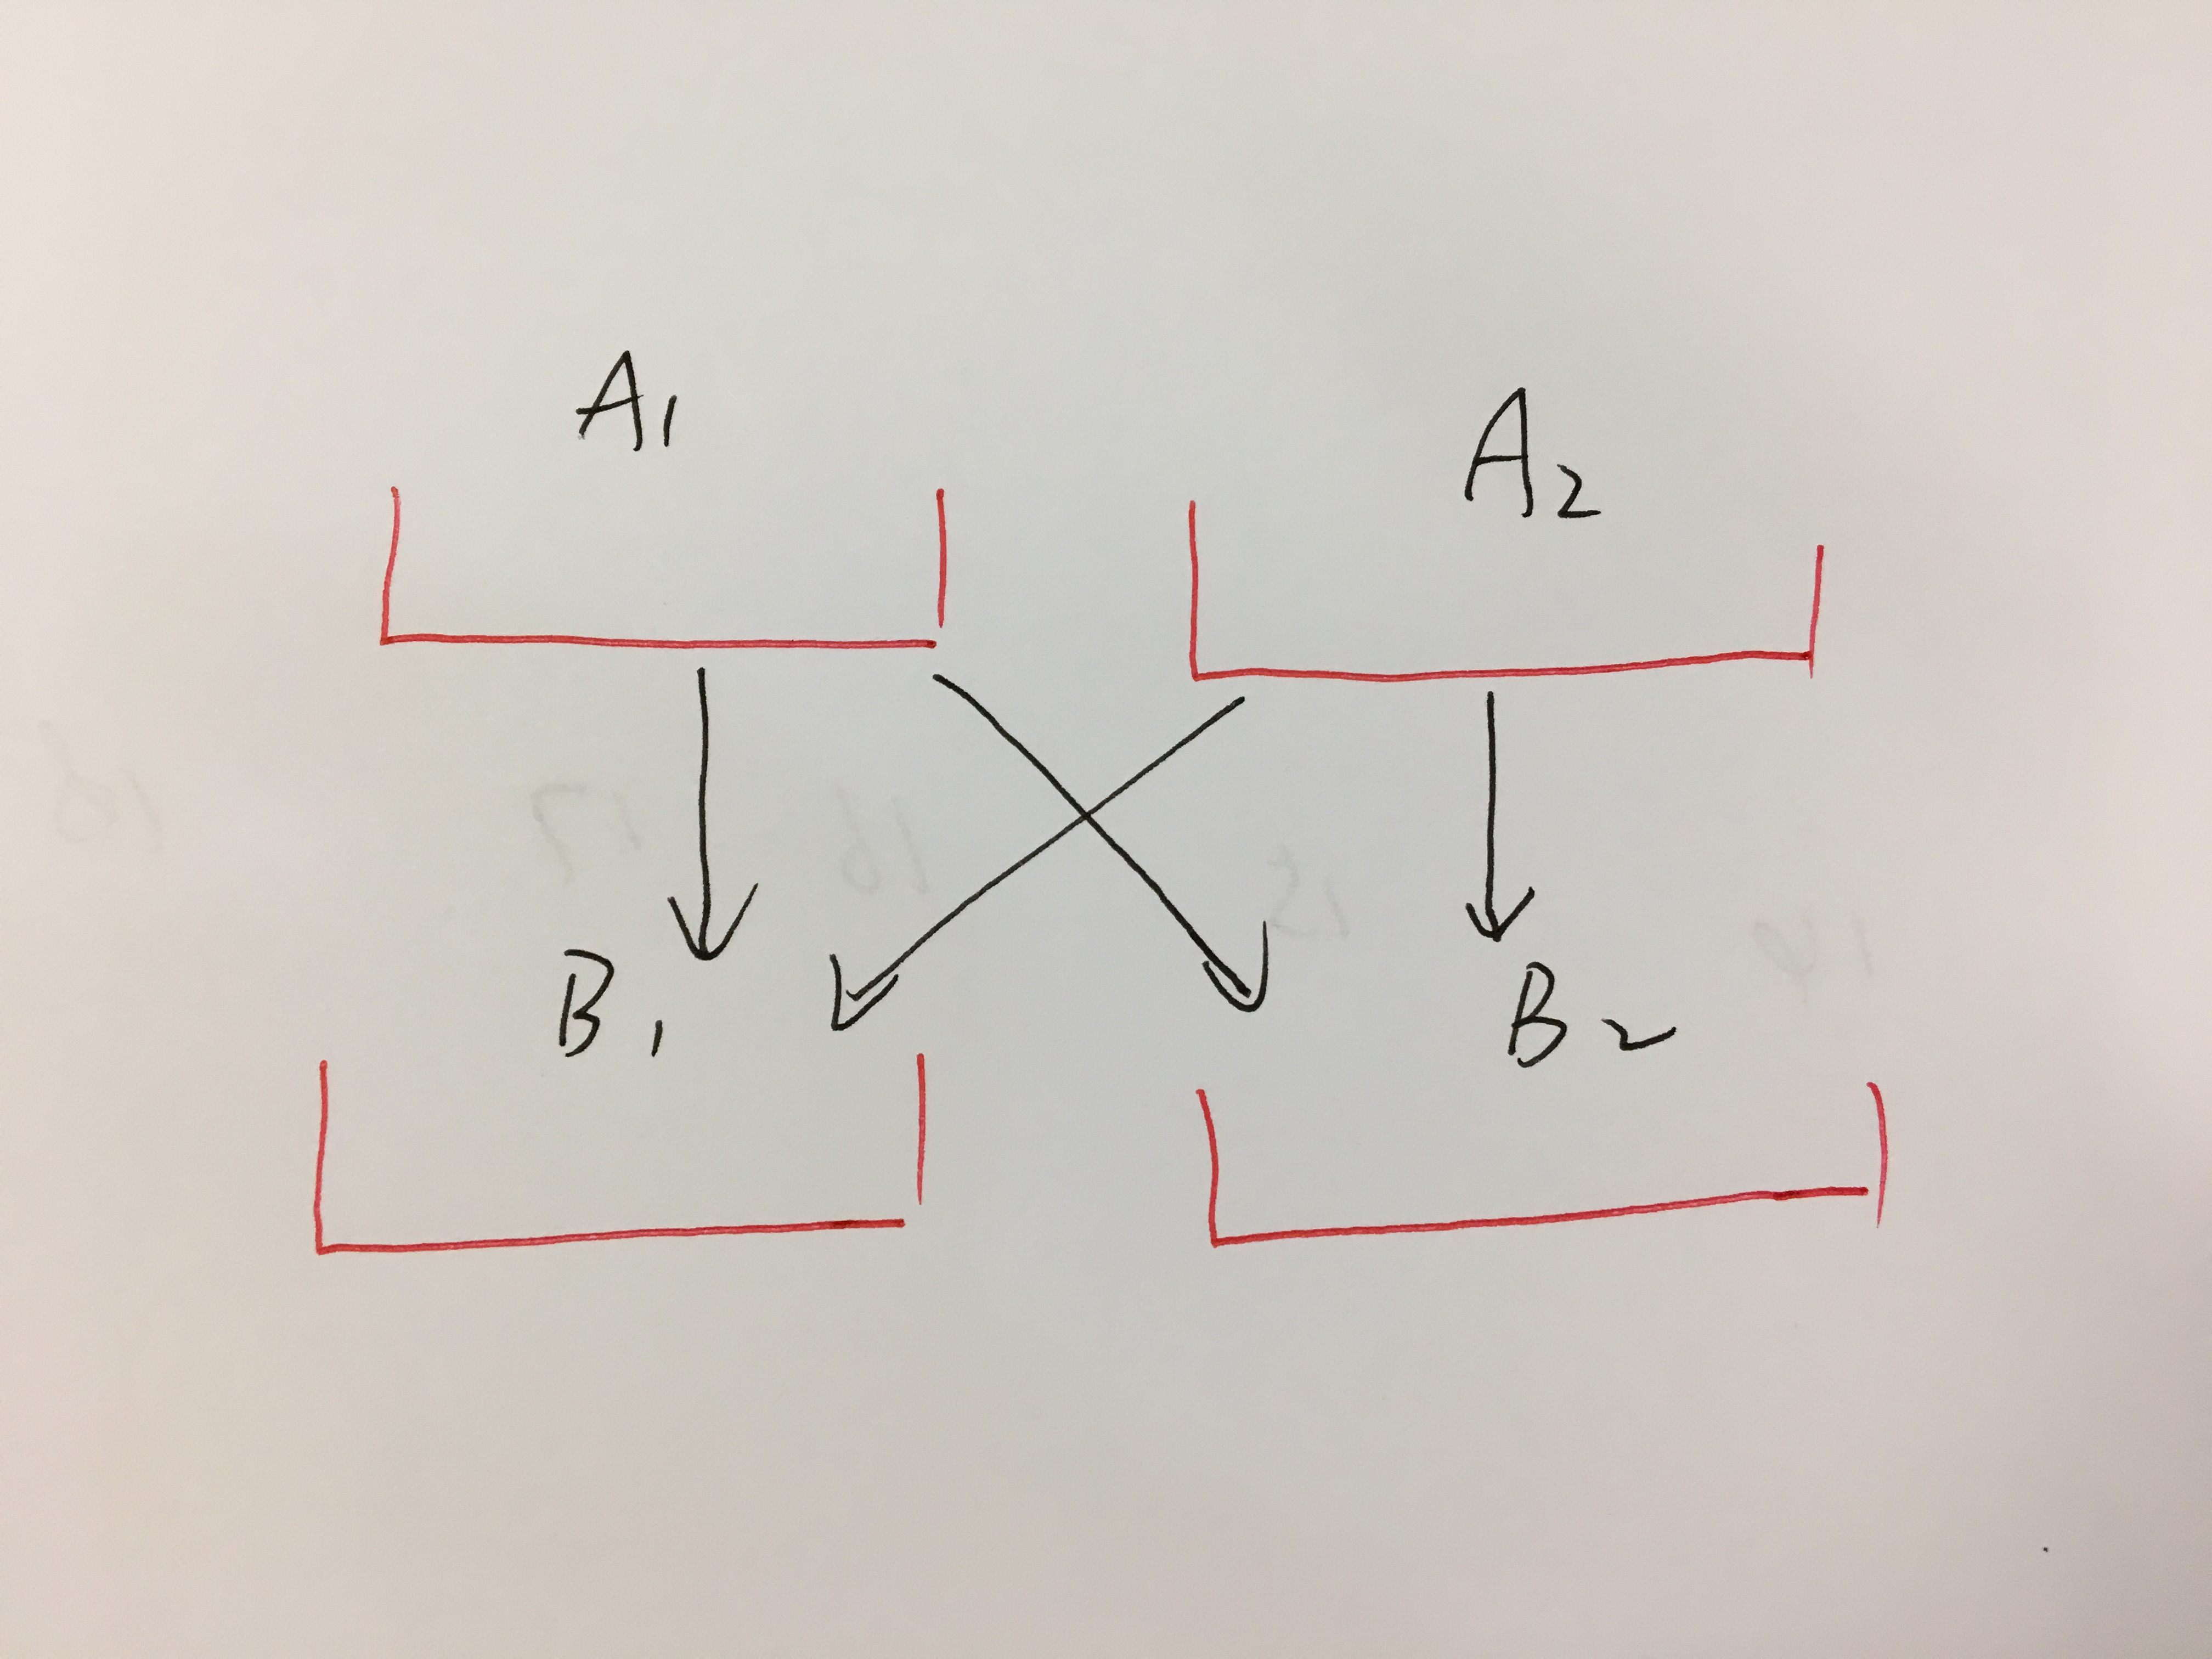
\includegraphics[width=2in]{11}\\
    If $j\oplus k=i$, we calculate together so we didn't need $n\times n$. We compute $\oplus$ first. $A_{1}-B_{2}$ and $A_{2}-B_{1}$ is same. And $A_{2}-A_{2}$ we can convert to same as $A_{1}-B_{2}$ because of $A\oplus X\oplus A\oplus Y=X\oplus Y$.
    So we just need to compute 2 parts($A_{1}-B_{1},A_{1}-B_{2}$). And we recursively do these operation. Combine we just merge same $i=j\oplus k$. So sum all $a_{j}b_{k}$. \\
    And the run time is $O(n\ log\ n)$.
  \end{enumerate}
  Done.
\end{solution}

\section*{DNA Pattern Recognition}
\paragraph{}
There are four possible bases in a DNA sequence: $A, G, C, T$. Suppose we have two DNA sequences $S$
and $P$ with length $n$ and $m$ where $\sqrt{n} < m < n − \sqrt{n}$. Design an efficient algorithm to find out the minimum
number of bases in $P$ that we have to change so that $P$ is a substring of $S$. For comparison, our algorithm
runs in $O(n\ log\ n)$ time.\\
For instance, $S =  AGCTAGGCTCT $, $P =  AAGTCTC $. The answer is $2$. We can change $P$ to
$ TAGGCTC $.\\
Hint: An application of FFT.
\begin{solution}

\end{solution}

\section*{2D Inversions}
\paragraph{}
Given an array of 2D pairs $A = a_{0},a_{1},\cdots,a_{n-1}$ where $a_{i}=(x_{i},y_{i}$, define $a_{i}>a_{j}$ as $x_{i}>y_{j}$ and
$y_{i}>y_{j}$ .
\begin{enumerate}[(a)]
  \item How many half-inversions are there? $a_{i}$ and $a_{j}$ are half-inverted if $i < j$, $x_{i} > x_{j}$ and $y_{i}\ge y' > y_{j}$
  where $y'$ is a fixed constant. Design an efficient algorithm. For comparison, our algorithm runs in $O(n\ log\ n)$
  time.
  \item How many cross-inversions are there? $a_{i}$ and $a_{j}$ are cross-inverted if $i <i'\le j$ and $a_{i}>a_{j}$ where $i'$
  is a fixed constant. Design an efficient algorithm. For comparison, our algorithm runs in $O(n\ log\ n)$ time.
  \item How many inversions are there? $a_{i}$ and $a_{j}$ are inverted if $i < j$ and $a_{i}>a_{j}$ . Design an efficient
  algorithm. For comparison, our algorithm runs in $O(n\  log^{2}\  n)$ time.
\end{enumerate}

\begin{solution}\
  \begin{enumerate}[(a)]
    \item  Use Divide-and-Conquer.
    \begin{itemize}
      \item Divide: separate list two pieces.
      \item Conquer: recursively sort $a_{i}$ based on $x_{i}$ and count inversions in each half.
      \item Combine: count inversions where $x_{i}>x_{j}$ and meanwhile satisfy that $y_{i}\ge y'>y_{j}$ are in different halves(merge and count), and returns sum of three quantities.($O(n\ log\ n)$).
    \end{itemize}
    The run time of algorithm is same as counting inversions. It's $O(n\ log\ n)$.
    \item Similar with question (a). But we don't recuisively count. We sort, merge and count inversion.
    \begin{itemize}
      \item Divide: separate list two pieces from $i'$.
      \item Sort: Sort $a_{i}$ based on $x_{i}$ in both two parts. ($O(n\ log\ n)$)
      \item Count: Merge and count. If $x_{i}>x_{j}$ and meanwhile satisfy that $y_{i}>y_{j}$ are in different halves, then the number of cross-inversions plus $1$. ($O(n)$).
    \end{itemize}
    The run time of algorithm is same as counting inversions. It's $O(n\ log\ n)$.
    \item Similar with question (a).
    \begin{itemize}
      \item Divide: separate list two equal pieces.
      \item Conquer: recursively sort $a_{i}$ based on $x_{i}$ count inversions in each half.
      \item Combine: count inversions where $x_{i}>x_{j}$ and meanwhile satisfy that $y_{i}>y_{j}$ are in different halves(merge and count), and returns sum of three quantities.($O(n\ log\ n)$).
    \end{itemize}
    The run time of algorithm is same as counting inversions. It's $O(n\ log\ n)$.
  \end{enumerate}
  Done.
\end{solution}

\end{document}
